\section{结果与讨论}

% Wide figures are declared before the running text so the compositor can fill each page.

\begin{figure*}[!tbp]
\begin{minipage}{\textwidth}
\centering
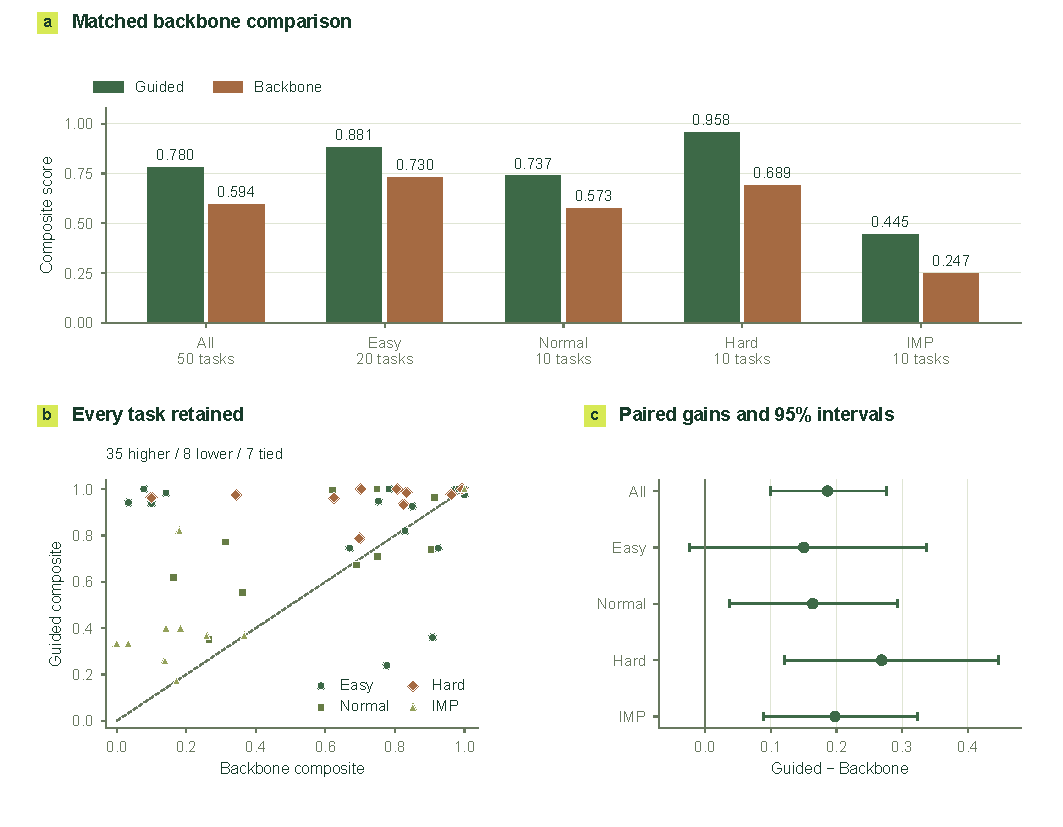
\includegraphics[width=\textwidth]{figures/bench_overview.pdf}
\caption{P2 主比较与逐题差异。a，Cloudra Guided 与同一 backbone 的 Standard 基线在全部 50 题及各难度层的整理后复合分；Easy 为 20 题，其余各 10 题。b，保留全部 50 个同题配对。c，配对均差与 100,000 次按任务整组 bootstrap 的 95\% 百分位区间。}
\label{fig:bench-overview}
\end{minipage}
\end{figure*}

\begin{figure*}[!tbp]
\begin{minipage}{\textwidth}
\centering
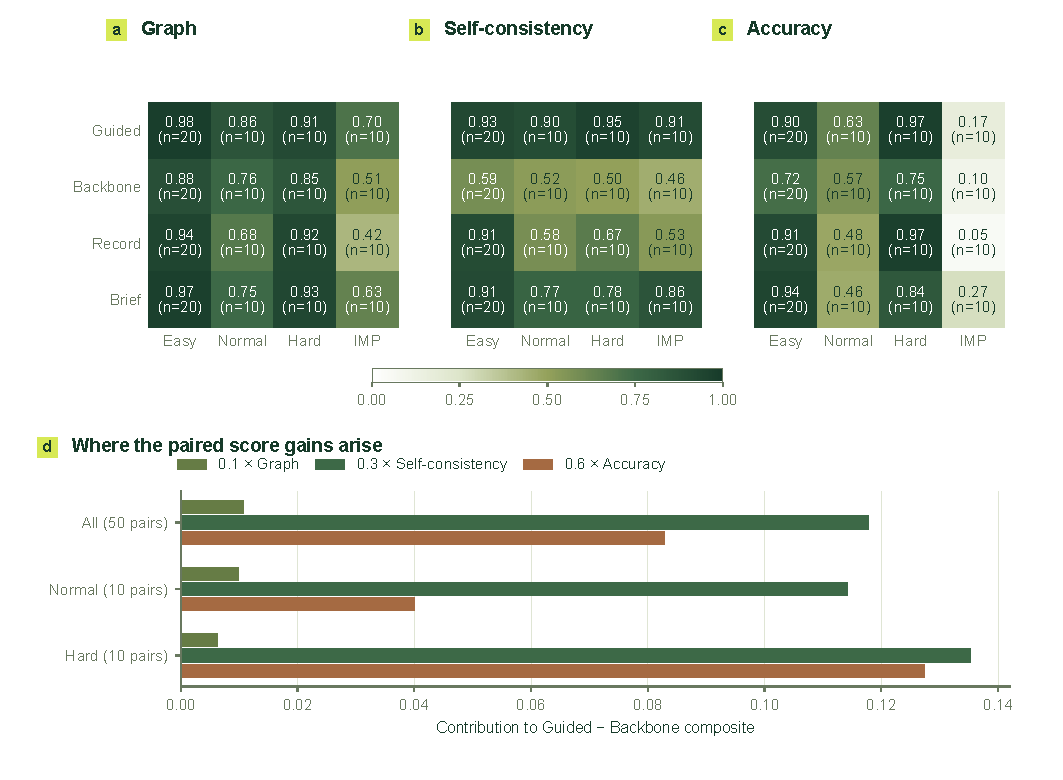
\includegraphics[width=\textwidth]{figures/bench_components.pdf}
\caption{全部200次整理后运行的三个评分层。a--c，各配置、难度层的Graph、自洽性与Accuracy均值；每配置总体50题，Easy为20题，其余各层10题。d，按固定0.1/0.3/0.6权重分解Guided相对Backbone的均差，全部、Normal与Hard分别使用完整50、10和10个配对。各运行分量由其自身研究材料与评分记录对齐至最终整理总分。}
\label{fig:bench-components}
\end{minipage}
\end{figure*}

\begin{figure*}[!tbp]
\begin{minipage}{\textwidth}
\centering
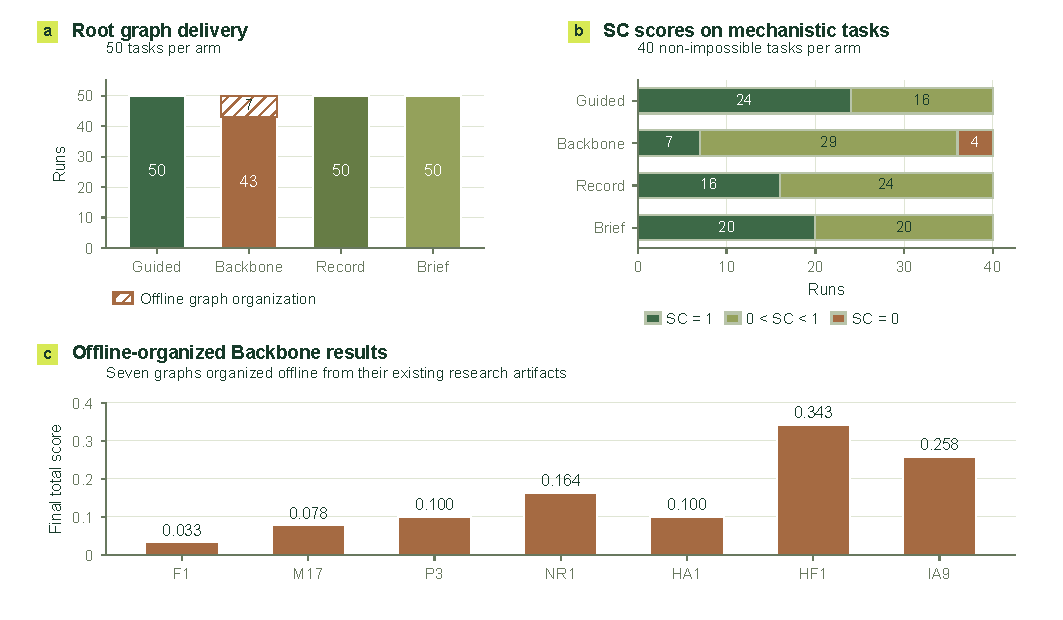
\includegraphics[width=\textwidth]{figures/bench_delivery.pdf}
\caption{运行期交付图与最终科学支持。a，每配置50题中的原始根图记录，Guided、Backbone、Record与Brief分别为50、43、50和50；斜线标记从运行自身材料离线组装的7份Backbone图，整理后每配置均为50份。b，每配置全部40道非Impossible题的自洽分布，区分SC=1、部分正分及SC=0；满分数依次为24、7、16和20，Backbone另有4题零分。c，7个未在运行中形成根图的Backbone任务整理后总分，范围0.0333至0.3425，均值0.1537。}
\label{fig:bench-delivery}
\end{minipage}
\end{figure*}

\begin{figure*}[!tbp]
\begin{minipage}{\textwidth}
\centering
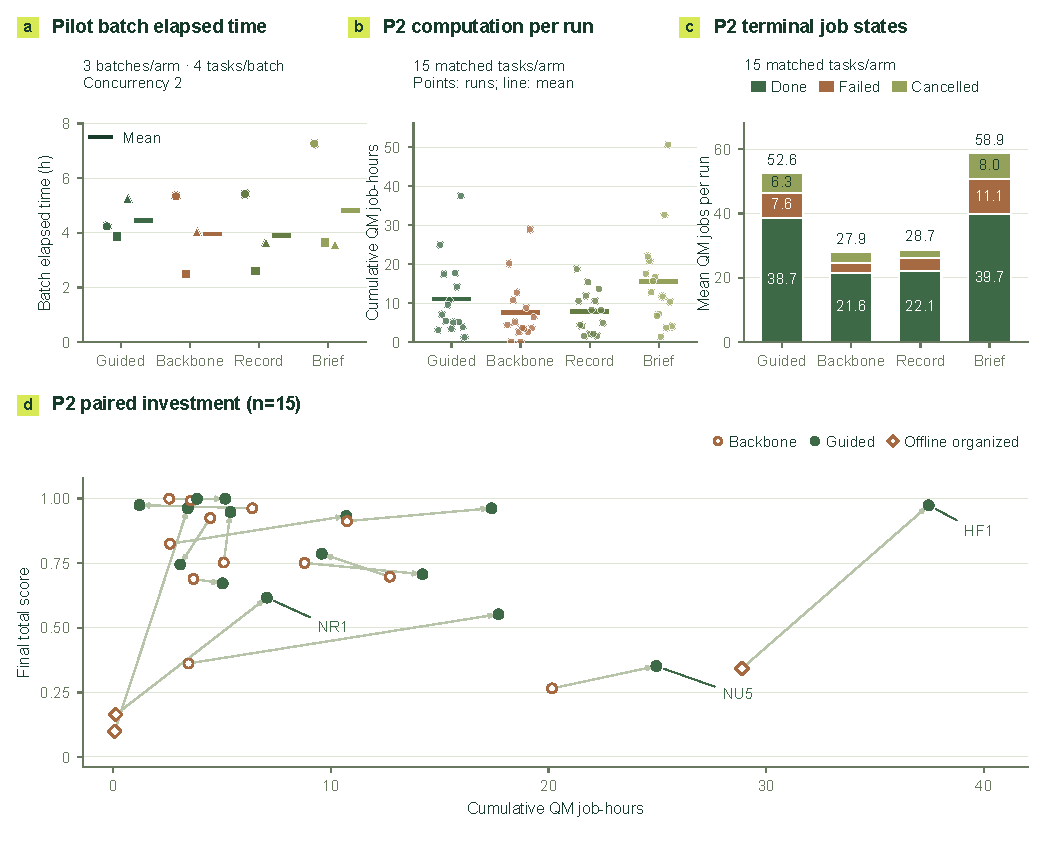
\includegraphics[width=\textwidth]{figures/bench_speed.pdf}
\caption{运行速度与计算投入。a，P1b 的 12 个真实批次，每配置 3 批，每批 4 题，并发为 2；点为观测批次，短线为均值。b，P2 四配置共同 15 题的逐运行累计 QM job-hours 及均值。c，同一任务集每运行的完成、失败和取消作业数量。d，Standard 与 Guided 同题的计算投入及整理后总分，箭头连接相同任务，菱形标记离线组装机理图的运行。}
\label{fig:bench-speed}
\end{minipage}
\end{figure*}

\begin{figure*}[p]
\begin{minipage}{\textwidth}
\centering
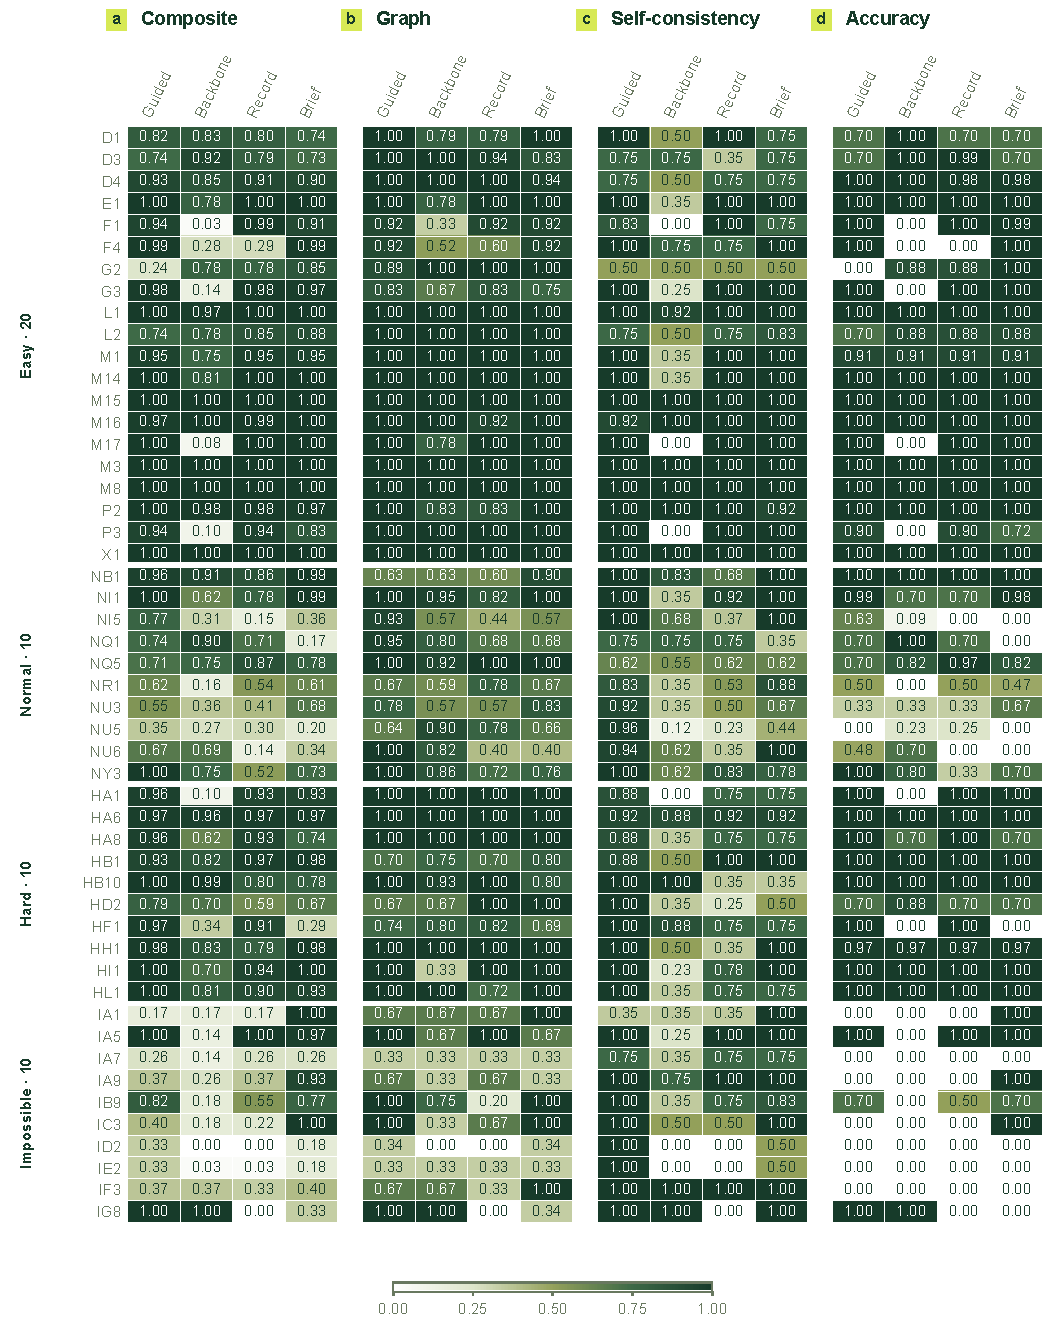
\includegraphics[width=\textwidth]{figures/bench_tasks_all.pdf}
\caption{CloudraBench全部50题、四配置的完整逐题成绩。四个评分块按相同顺序展示综合分、Graph、自洽性与Accuracy，色标统一为0--1，800格全部呈现。数值保留两位小数，来源表保留完整精度。}
\label{fig:bench-tasks}
\vspace{6pt}
\end{minipage}
\end{figure*}

\begin{figure*}[!tbp]
\begin{minipage}{\textwidth}
\centering
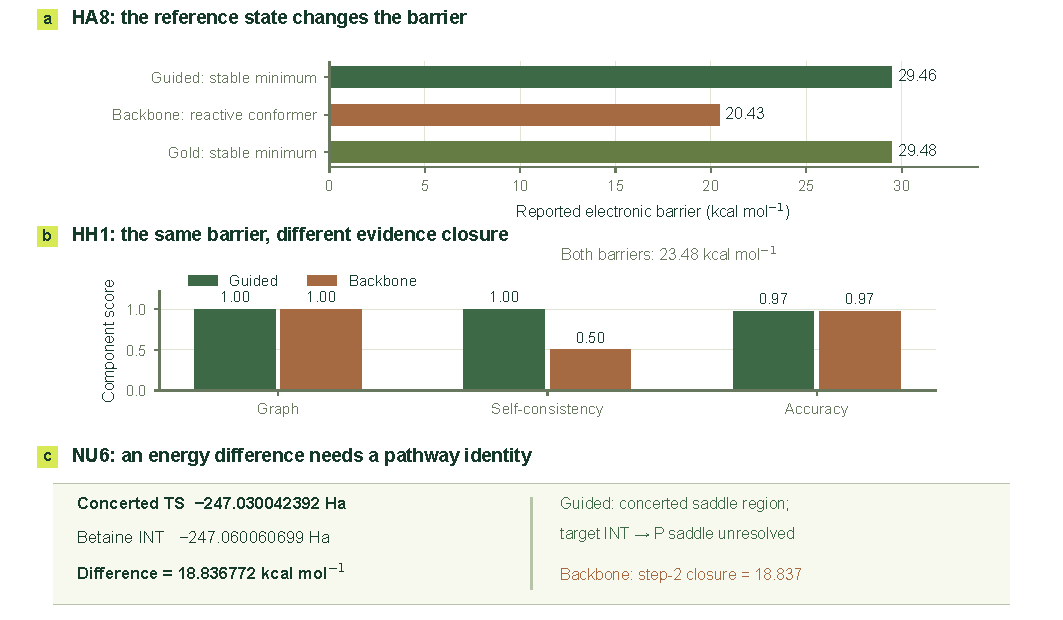
\includegraphics[width=\textwidth]{figures/bench_cases.pdf}
\caption{计算结果的科学归属。a，HA8 分别采用稳定极小值与反应性构象作参照的声明能垒，与 campaign Gold 并列。b，HH1 两组均给出 23.48 kcal/mol 能垒且准确度接近，自洽证据分不同。c，NU6 两个已记录能量之差为 18.836772 kcal/mol；Guided 将其保留为 concerted 鞍点区域的代价，并将目标闭环鞍点留为未解决，Standard 则将 18.837 声明为第二步闭环能垒。计算细节与路径文字取自归档证据记录。}
\label{fig:bench-cases}
\end{minipage}
\end{figure*}

\begin{figure*}[!tbp]
\begin{minipage}{\textwidth}
\centering
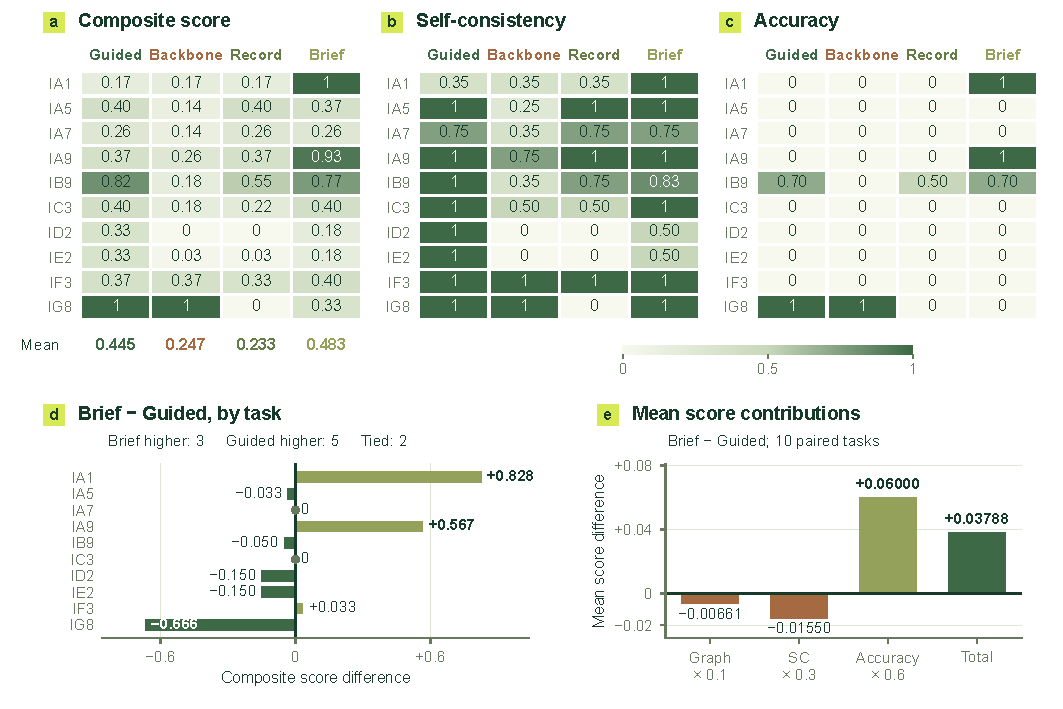
\includegraphics[width=\textwidth]{figures/bench_imp.pdf}
\caption{Impossible层的逐题对照与Brief--Guided差异。a--c，全部10题、四配置的完整整理总分、自洽性和Accuracy，色标统一为0--1。d，Brief相对Guided的逐题总分差，均差+0.03788集中于IA1与IA9，IG8呈相反结果；Guided赢5题、Brief赢3题、2题持平。e，按既定权重分解均差，Accuracy贡献+0.06000、Graph贡献$-0.00661$、自洽性贡献$-0.01550$，细微加总差异来自保存总分的舍入；任务bootstrap的95\%区间为$-0.188$至+0.284，逐题科学声明见下文分析。}
\label{fig:bench-imp}
\end{minipage}
\end{figure*}

\begin{figure*}[!tbp]
\begin{minipage}{\textwidth}

\centering
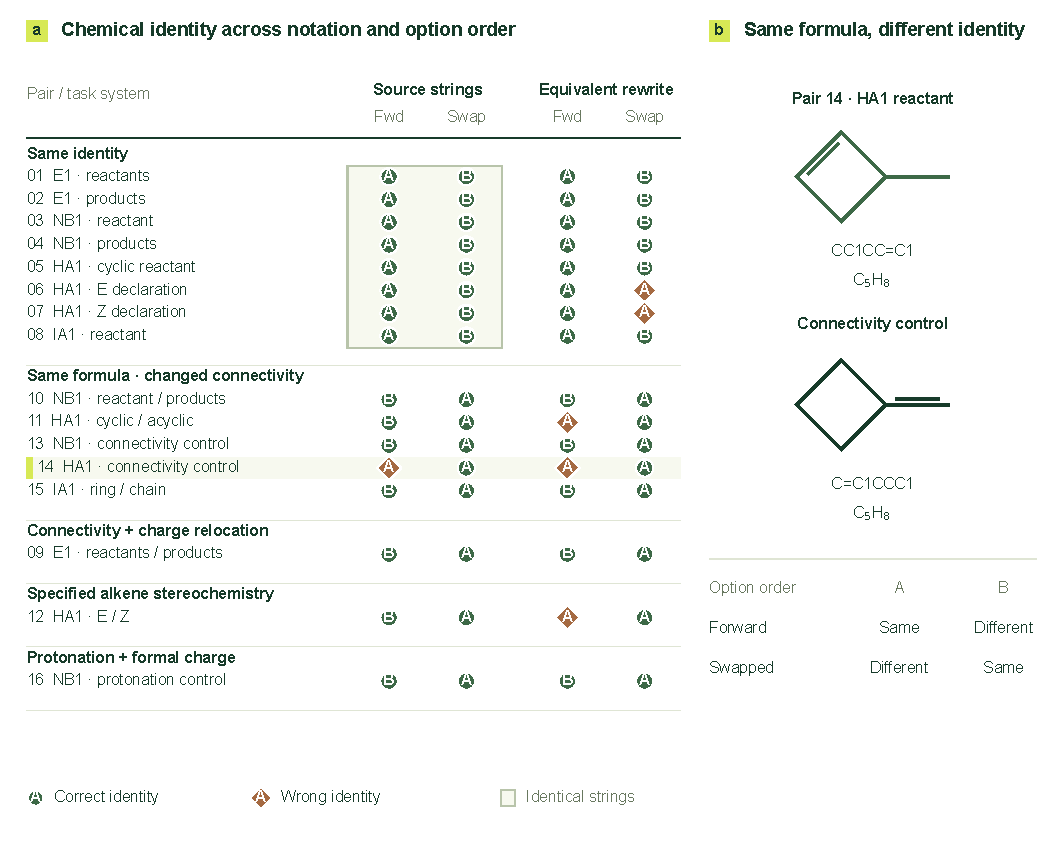
\includegraphics[width=\textwidth]{figures/fig06.pdf}
\caption{分子表示与选项顺序下的化学身份判断。16 对分子各包含四种输入条件；圆形和菱形分别表示正确与错误，内部字母保留模型实际回答。浅色区域为相同字符串条件。右侧显示第 14 对的两种 C\textsubscript{5}H\textsubscript{8} 连接结构及选项含义。}
\label{fig:06}
\end{minipage}
\end{figure*}

\begin{figure*}[!tbp]
\begin{minipage}{\textwidth}
\begin{minipage}[t]{.65\textwidth}
\vspace{0pt}
\centering
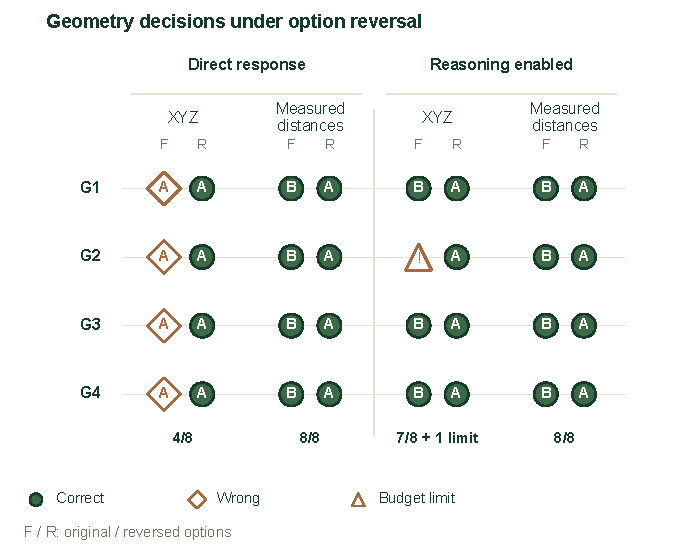
\includegraphics[width=\linewidth]{figures/fig07.pdf}
\caption{坐标输入与测量距离输入下的几何判断。四个源结构分别在直接回答和开启思考条件下比较，每种条件均包含原始（F）与交换（R）选项顺序。圆形表示正确，菱形表示错误，三角形表示达到输出预算；内部字母保留实际回答。}
\label{fig:07}
\end{minipage}\hfill
\begin{minipage}[t]{.31\textwidth}
\vspace{0pt}
\centering
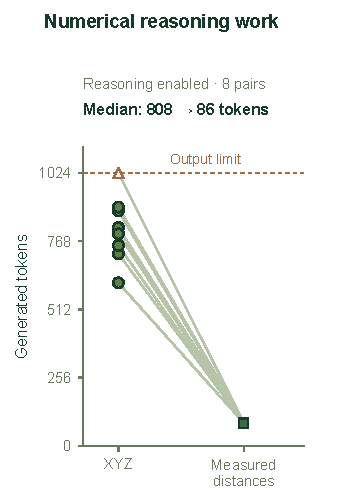
\includegraphics[width=\linewidth]{figures/fig08.pdf}
\caption{开启思考时的生成 token 数。每条线连接同一源结构、同一选项顺序下的笛卡尔坐标输入与测量距离输入，共八组配对比较。虚线表示输出上限。}
\label{fig:08}
\end{minipage}
\end{minipage}
\end{figure*}

\begin{figure*}[!tbp]
\begin{minipage}{\textwidth}
\centering
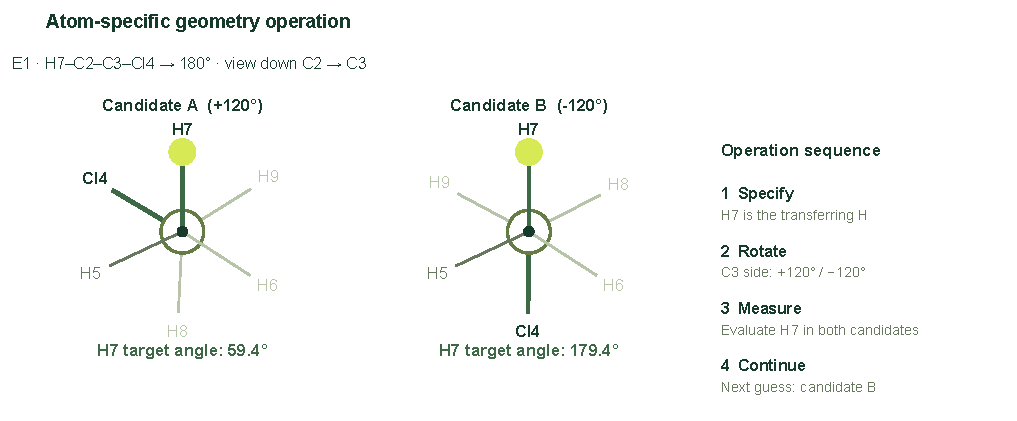
\includegraphics[width=.92\textwidth]{figures/fig09.pdf}
\caption{E1 中面向指定目标的几何操作。Newman 投影保留原候选坐标沿 C2\(\to\)C3 观察时的方向。H7 为指定的转移原子；候选 A、B 的目标角分别为 59.4° 和 179.4°。投影旁列出相应操作顺序。}
\label{fig:09}
\vspace{5pt}
\begin{minipage}[t]{.48\textwidth}
\vspace{0pt}
\centering
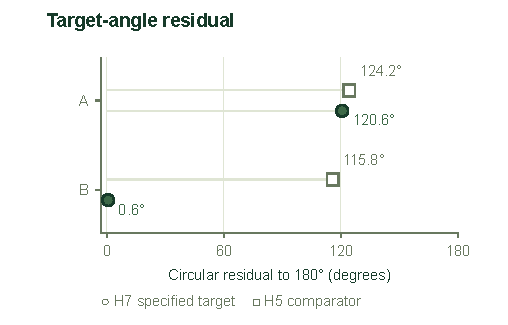
\includegraphics[width=\linewidth]{figures/fig10.pdf}
\caption{候选 A、B 相对指定 180° 目标的圆周角残差。H7 为指定目标原子，H5 为比较原子。}
\label{fig:10}
\end{minipage}\hfill
\begin{minipage}[t]{.48\textwidth}
\vspace{0pt}
\centering
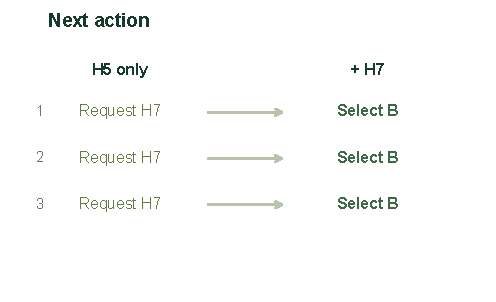
\includegraphics[width=\linewidth]{figures/fig11.pdf}
\caption{三种局部选项排列下的后续动作。仅提供 H5 测量值时，模型请求 H7 测量；补充 H7 后，模型选择候选 B。}
\label{fig:11}
\end{minipage}
\end{minipage}
\end{figure*}

\begin{figure*}[!tbp]
\begin{minipage}{\textwidth}
\centering
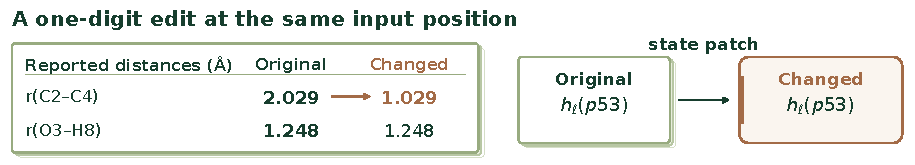
\includegraphics[width=.92\textwidth]{figures/fig12.pdf}
\caption{对单个报告距离的干预。一次数字修改将 C2–C4 距离从 2.029 改为 1.029 Å，O3–H8 保持 1.248 Å。在指定层，将原始输入中 token 位置 53 的残差状态替换到修改后输入的运行中。token 位置从零计数。}
\label{fig:12}
\vspace{4pt}
\centering
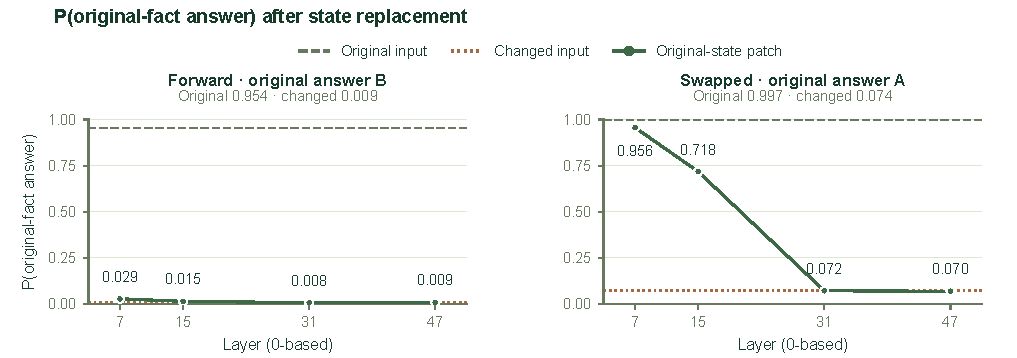
\includegraphics[width=.92\textwidth]{figures/fig13.pdf}
\caption{状态替换后原始事实答案的概率。曲线显示原始顺序（答案 B）与交换顺序（答案 A）下，原始事实答案在完整词表中的概率质量，包含无前导空格与带前导空格的 token 写法。水平线为原始输入与修改后输入的基线。层号从零计数。}
\label{fig:13}
\vspace{4pt}
\centering
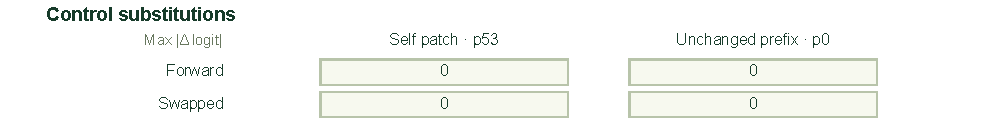
\includegraphics[width=.92\textwidth]{figures/fig14.pdf}
\caption{状态干预实验的对照替换。在 p53 进行同状态自替换，以及在 p0 替换未改变的前缀，两种选项顺序下均保持全部词表 logits 不变。表中报告 logit 差值绝对值的最大值。token 位置从零计数。}
\label{fig:14}
\end{minipage}
\end{figure*}

\begin{figure*}[!tbp]
\begin{minipage}{\textwidth}

\begin{minipage}[t]{.48\textwidth}
\vspace{0pt}
\centering
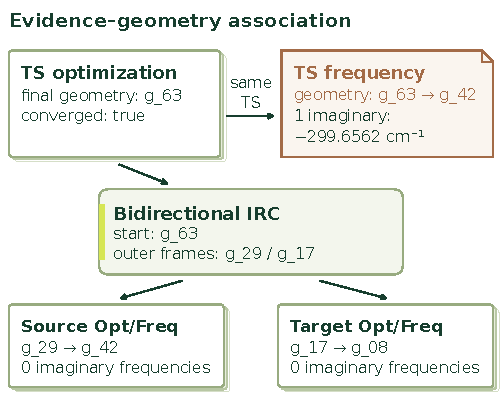
\includegraphics[width=\linewidth]{figures/fig15.pdf}
\caption{E1 源链中的证据与几何关联。受控输入将频率计算的几何引用从 g\_63 改为 g\_42，同时保持局部终止、收敛、能量和频率数值。图中保留从过渡态优化、双向 IRC 到端点优化与频率计算的关联。}
\label{fig:15}
\end{minipage}\hfill
\begin{minipage}[t]{.48\textwidth}
\vspace{0pt}
\centering
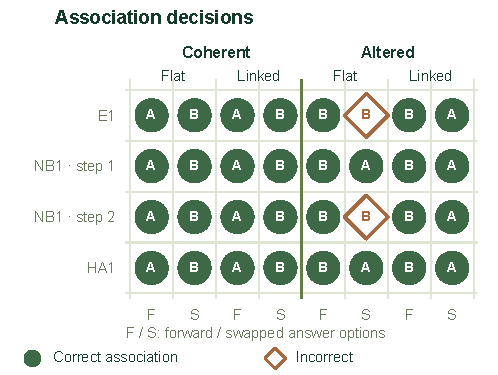
\includegraphics[width=\linewidth]{figures/fig16.pdf}
\caption{四条源链共 32 个输入的关联判断，交叉比较一致或修改后的关联、平铺或关联式表示，以及原始（F）或交换（S）答案顺序。字母保留已保存的 A/B 回答；圆形表示正确关联，菱形表示错误关联。}
\label{fig:16}
\end{minipage}
\end{minipage}
\end{figure*}

\begin{figure*}[!tbp]
\begin{minipage}{\textwidth}
\centering
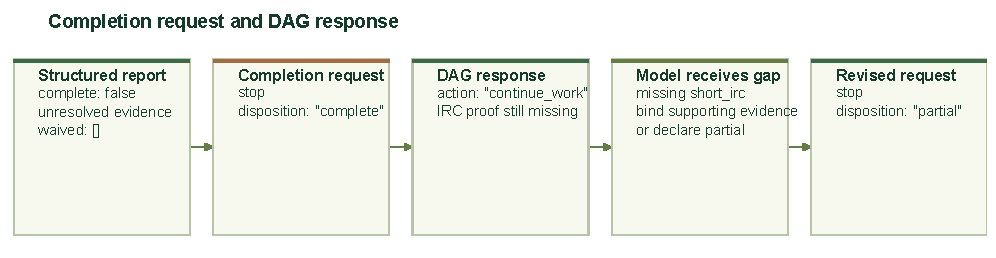
\includegraphics[width=.96\textwidth]{figures/fig17.pdf}
\caption{原始 IA1 轨迹中的完成请求与 DAG 反馈。报告仍有未解决的证据后，模型请求完成；系统指出缺少 short\_irc 证明并向模型反馈，随后模型改为请求部分完成。}
\label{fig:17}
\end{minipage}
\end{figure*}

\subsection{用化学对象表达一个两步反应机理}
\label{sec:ni1-chemical-objects}

Guided 的 NI1 运行研究甲胺对甲醛的加成，以及随后脱水形成亚胺—水复合物的过程（图~\ref{fig:ni1-chemical-objects}）。物种对象保存优化后的反应物复合物、半缩胺中间体和产物复合物，两个步骤对象分别通过一阶鞍点连接相邻物种。图中的结构和电子能全部来自该次运行自身的 B3LYP-D3(BJ)/def2-SVP 气相计算，电荷为0，自旋多重度为1。

加成鞍点具有唯一的虚频 $-1481.06$ cm$^{-1}$，相对反应物复合物的电子能垒为28.12 kcal/mol。两个方向的短 IRC 外帧分别经几何优化和频率计算到达反应物复合物与半缩胺中间体，两者均无虚频。脱水鞍点具有唯一的虚频 $-1796.84$ cm$^{-1}$，两个方向同样得到半缩胺和亚胺—水复合物。每次 IRC 均在两个方向各追踪24个点后达到点数上限，随后用独立端点计算确定相应极小值。

脱水能垒还说明一个物种对象为何需要保存多个几何构象。该步骤实际 IRC 一侧到达的半缩胺极小值，比运行中找到的最低半缩胺构象高0.71 kcal/mol。以局部 IRC 端点为参考的能垒为57.21 kcal/mol，以最低构象为参考则为57.92 kcal/mol。步骤对象因此同时保存真实路径端点和计算能垒时采用的稳定参考构象。两个构象间的互变路径仍待计算。SI 第S4节给出绝对能量、原生计算位置和可复现的绘图输入。





















\subsection{端到端基准评估}

CloudraBench 衡量端到端机理计算能力：构建候选机理、完成所需量子化学计算，并得出符合任务要求的正结论或负结论，其中包括判断允许方法下目标的物理存在性。下文报告最终整理后的综合分及图结构、自洽性与准确度分量。离线整理从每次运行自身的研究材料组装机理图，并关联该运行已有的评分记录，得到200次运行全部三项分量与综合分，整体均分为0.7051。图~\ref{fig:bench-overview}至图~\ref{fig:bench-tasks}报告运行期根图生成情况、TS—IRC—端点证据，以及结果与任务答案的符合程度。

\subsubsection{同一模型下，Cloudra提高了端到端机理计算得分}

Guided 的综合均分为0.7930，Standard 为0.5814。50道题逐题配对的平均增益为0.2116，95\%任务 bootstrap 区间为[0.1290, 0.2985]。Guided 在36题中更高、7题中更低、7题持平，配对差值的中位数为0.1142（图~\ref{fig:bench-overview}）。



各组最低分十题的均值也有差别：Guided 为0.3221，Standard 为0.0930。



最一致的改善出现在 Hard 立体化学任务。Guided 均分为0.9577，Standard 为0.6888，配对增益为0.2689 [0.1213, 0.4459]，十题中 Guided 全部更高。这些任务要求将每个能垒和计算路径归到相应立体异构体或竞争通道。

Normal 任务中，Guided 均分为0.7370，Standard 为0.5731，增益0.1640 [0.0365, 0.2922]，7题更高、3题更低。Easy 均分分别为0.9125和0.6989，但配对差值中位数为0.0500，其分布与 Hard 中广泛为正的改善不同。Impossible 均分分别为0.4451和0.2473；这组分数取决于运行是否回答了题目所要求的方法受限负结论，因而在后文单独分析。





\subsubsection{自洽性对综合分增益的贡献最大}

三项分数分别评价计算的不同内容（图~\ref{fig:bench-components}）。Graph 衡量交付物中所要求物种与步骤的覆盖及身份；Self-consistency 衡量鞍点、频率、IRC起点与端点优化/频率之间的支持关系；Accuracy 衡量结果与任务数值或负目标的符合程度。因此，一次运行可能给出接近参考的数值，而路径仍待补证；也可能完成了回答另一个研究问题的局部自洽计算。

全部50个 Guided--Standard 配对中，平均增益的加权图结构贡献为+0.0108，自洽性贡献为+0.1179，准确度贡献为+0.0829，合计对应综合增益0.2116。Normal与Hard的全部20题均差为0.2164，图结构、自洽性与准确度分别贡献+0.0080、+0.1247和+0.0837。



其中10道Normal题的三项贡献为+0.0098、+0.1141和+0.0400，10道Hard题为+0.0063、+0.1353和+0.1274。Hard中准确度与自洽性的加权改善幅度相近。



HH1给出了直接例子。Guided 与 Standard 均交付联萘消旋能垒23.48 kcal/mol，接近参考23.01 kcal/mol；两者图结构均为1，准确度均约0.973。自洽性分别为1.0和0.5，对应综合分0.9838和0.8338。归档的 Standard 研究已有候选通道和 IRC 输入；所要求的端点连接仍待证实；Guided 将路径证据关联至相应鞍点及端点。HI1呈现类似结果：两组准确度均约为1，自洽性由0.2333提高至1.0，综合分由0.7032提高至0.9999。因此，确定鞍点实际连接哪些极小值，仍需补充IRC及端点计算。





\subsubsection{交付文件与分级科学支撑分别记录}

运行期是否生成根图，与原运行中找到的物理证据分别记录（图~\ref{fig:bench-delivery}）。原运行中，Standard在50题中交付43份根图，Guided、Record与Brief-errors各交付50份。Standard需离线重建根图的7题为F1、HA1、HF1、IA9、M17、NR1和P3。离线整理从对应运行已有研究材料组装其机理图，最终各配置均形成完整50题记录。恢复这7份Standard记录，使基线已完成的研究得到相应评分，避免仅因缺少根交付文件而低估基线，从而使组间比较更保守。

Standard这7题整理后均分为0.1537，Guided在相同任务上的均分为0.8285，贡献了两组总净差的44.7\%；其逐题分数范围为0.0333至0.3425。计算结果和候选描述可能已经留在运行记录中，而所要求的路径或比较结论仍未完成；离线整理将这些已有内容恢复出来，用于评价。







各配置40道非Impossible任务中，Guided有24题的自洽连续分恰好为1（60.0\%）、16题获得部分正分；Standard有7题满分（17.5\%）、29题部分正分、4题零分；Record为16题满分（40.0\%）、24题部分正分；Brief-errors有20题满分（50.0\%）及20题部分正分。图~\ref{fig:bench-delivery}并列展示完整证据分布与单独记录的运行期根图交付数。

上述百分比表示已交付对象的自洽性分量满分比例。整道题的科学完成率还要求每个请求物种与步骤均有物理支持。归档运行指标覆盖已交付或智能体选定的对象；针对全部请求对象的统一核查仍待完成。SI 第S4节说明这些记录各自覆盖的范围。

\subsubsection{工具相同时，Guided得分仍高于Record}

Record的全50题均分为0.6918，Brief-errors为0.7541。Guided相对Record高0.1012 [0.0396, 0.1695]，28题更高、7题更低、15题持平。Normal与Hard全部20题均差为0.1468，其中图结构贡献+0.0083、自洽性+0.0919、准确度+0.0466。最大的分量差异来自自洽性，即支持所报告步骤的频率、IRC及端点计算。





\subsubsection{研究批次耗时与量子化学作业时长}

图~\ref{fig:bench-speed}并列展示重复实验的耗时和 P2 可获得的计算投入。重复实验的测量单位是一个四题批次，批内并发度为2，每种配置实际观察3个批次。Guided、Standard、Record 和 Brief-errors 的平均批次耗时分别为4.451、3.958、3.894和4.827小时。Guided 平均比 Standard 长12.5\%，比 Brief-errors 短7.8\%。图中保留12个真实批次点及原始运行结果所对应的变异。这一测量包含批次的研究生命周期、计算等待及结果返回后的继续研究。

P2投入统计覆盖四组共有的15道深挖任务。Guided 每题使用11.08 job-hours，Standard 为7.55，Record 为7.88，Brief-errors 为15.59；对应最终综合均分分别为0.8124、0.6495、0.7360和0.7273。相对 Standard，Guided 累计计算时长多46.7\%，均分高0.1629；相对 Brief-errors，累计计算时长少28.9\%，均分高0.0851。在15个配对任务中，Guided 有7题同时比 Brief-errors 使用更少累计计算时长并得到更高分。



共同任务中，Guided 记录789个量子化学作业，Standard 为419，Record 为431，Brief-errors 为883；其中失败作业分别为114、45、62和167，取消作业另行记录。NU3、NU5、NU6和NR1四道困难研究的16次运行共使用163.5 job-hours，占可用63条投入档案673.82 job-hours的24.3\%。这四项研究追加尝试后，仍有步骤待解决。在归档的 Standard 缺图案例中，计算还可能晚于研究会话结束，后续结果因而留在已经结束的研究会话之外。

Guided 相对 Brief-errors 的总体增益为0.0388，区间为[$-0.0317$, 0.1076]，26题更高、10题更低、14题持平。比较随研究要求改变：Guided 在 Normal 中平均高0.1514，在 Hard 中高0.1295，而 Brief-errors 的 Impossible 均分更高。









\subsubsection{共同数值子集中的未封顶电子能垒误差}

为用化学单位表达数值偏差，我们从归档原生日志的过渡态与反应物参考电子能重新计算能垒。四组共有的数值子集包含23道正结论任务中的26条参考边：各组均可恢复相应数值，且已有分量与最终发表记录一致。分析保留原评分器的选边结果，逐边对比冻结的题目参考值，每条边在每组中计入一次，能量换算沿用第2节定义。表~\ref{tab:uncapped-barrier-errors}给出未封顶误差。

\begin{table}[tbp]
\centering\small
\caption{四组共同26条参考边的未封顶电子能垒误差，单位为 kcal/mol。}
\label{tab:uncapped-barrier-errors}
\begin{tabular}{lrrr}
\toprule
组别 & MAE & RMSE & 绝对误差中位数 \\
\midrule
Guided & 1.17 & 2.86 & 0.057 \\
Standard & 1.90 & 5.09 & 0.057 \\
Record & 1.58 & 5.71 & 0.073 \\
Brief-errors & 1.13 & 2.31 & 0.099 \\
\bottomrule
\end{tabular}
\end{table}

这些误差保留了综合评分中 Accuracy 惩罚封顶所压缩的较大偏差。在该子集中，Guided 的 MAE 和 RMSE 均低于 Standard，Brief-errors 的两项指标最低。该子集描述可恢复的数值答案，频率与反应路径的物理支持由自洽性分量另行衡量。SI 第S4节列出逐条数值、相对53条正结论数值参考边的覆盖情况，以及具有额外 Gold 输入方法与介质佐证的更小子集；数值排序随覆盖范围变化。

\subsubsection{逐题比较能垒、路径与计算证据}

图~\ref{fig:bench-tasks}展示全部50题、四种配置及完整评分分量。NB1和NI1也展示了多步机理计算中的得分情况。NB1中，Guided、Standard和Brief-errors分别为0.9628、0.9128和0.9900，Guided与Brief-errors的自洽性均为1；NI1中，Guided为0.9958，Standard为0.6196，自洽性分别为1和0.35。与此同时，NQ5中Record高于Guided，NU3中Brief-errors更高。

归档记录解释了几个具体能垒差异（图~\ref{fig:bench-cases}）。HA8中，Guided 给出29.46 kcal/mol，Standard 给出20.43 kcal/mol，参考为29.48 kcal/mol。档案将9.03 kcal/mol的差别追溯至能量参照：Guided 采用最低 all-s-trans 反应物极小值，Standard 采用反应性 cisoid 构象。



IRC确定鞍点连接的局部结构；报告活化能时，则采用题目规定的稳定极小值作能量参照。



NU6显示路径身份也可能在计算后改变。Guided 记录的 concerted 鞍点能量为$-247.030042392$ Ha，betaine极小值为$-247.060060699$ Ha，两者差为18.836772 kcal/mol。Guided 将其描述为经过 concerted 鞍点区域的能量代价，并将目标 betaine至产物闭环鞍点保留为待解决状态；Standard 则将18.837 kcal/mol交付为第二步闭环能垒。两份报告将这一几乎相同的能差归给了不同过程。Guided 从 betaine 插值结构和受约束扫描峰出发的尝试，释放约束后反复回到直接反应物至产物的鞍点区域。因此，需要根据优化后的几何和路径重新判断实际找到哪个鞍点。



G2中，Guided 得分0.2389，Standard 为0.7769。Guided 原生日志支持约0.845 kcal/mol的双氢转移能垒。伴随边的数值能垒声明三次被拒绝后，Agent 删除了数值字段；Supervisor 反馈促使其恢复字段，第四次拒绝及随后的鞍点证据检查后，最终图再次删除数值能垒以及鞍点能量、日志绑定。数值仅保留在文字说明中，准确度为0。Brief-errors 保留了相应数值结果，得分0.8500。

D1、D3和L2中0.7的准确度来自既定数值偏差罚分上限。D1与 Standard 的能垒差追溯至反应物构象参照，D3则主要来自鞍点能量差。L2区分反应性cZc与更低的tZt参照；Standard 已交付相应的18.99与28.28 kcal/mol两种能垒，参考匹配选中了前者。补充信息给出了这五题各工作流的最终分项得分、原生证据与交付记录。





\subsubsection{Impossible任务区分局部证据与目标负结论}

Impossible 组考察在 xTB/PM7 限制下能否得到题目规定的方法受限结论。Brief-errors 均分为0.4829，Guided 为0.4451，Standard 为0.2473，Record 为0.2325（图~\ref{fig:bench-imp}）。Brief-errors 相对 Guided 赢3题、负5题、平2题。其平均高0.0379，集中于特定答案：IA1贡献+0.8283，IA9贡献+0.5666；相反，IG8中 Guided 的结果在 Brief-errors减Guided方向贡献$-0.6661$。

IA1涉及环丁二烯方形几何的自同分异构目标，Brief-errors 的图结构、自洽性和准确度均为1，Guided 准确度为0。IA9涉及二氧杂环丁烷热分解，两组自洽性均为1，准确度分别为1和0。铬二聚体目标IG8则呈相反的准确度排序。在 Brief-errors 与 Guided 准确度相同的其余7题中，Brief-errors 平均低0.0500。



其 Impossible 总体优势分解为图结构$-0.0066$、自洽性$-0.0155$、准确度+0.0600：更高均分来自特定任务的目标结论，而 Guided 在另外一些任务中保留了更充分的局部支持。



全部40次 Impossible 运行中，4次准确度为1，14次同时具有自洽性1与准确度0。例如，Guided 与 Brief-errors 在IA5、IC3和IF3中均得到自洽性1和目标负结论准确度0；在兼含正负步骤的IB9中，两者准确度均为0.7。

保存的 Brief-errors/IC3图提供了科学报告层面的具体例子。图中将最低开壳层单重态及相应状态转换边标记为不可达，拒绝给出所求单重态—三重态能隙；已经计算的闭壳层单重态仍作为独立表征分支保留，两个方法依赖的相对能量被明确排除在目标能隙之外。该运行保留了有效探索结果，同时将这些结果明确限定于已经计算的闭壳层态；其最终准确度分仍为0。这一明确拒绝与准确度得分之间的差异将在讨论中分析。


















\subsection{分子识别、原子间距比较与片段旋转}


下文检验模型能否区分分子身份、比较指定原子间距、识别计算记录中错误的几何引用，以及找出尚缺的 IRC 计算。分子结构和计算记录取自归档研究轨迹；采用 Qwen3.8:27b 的局部对照分别改变输入信息、答案顺序及选定的内部状态，观察这些变化对各项判断的影响。

\subsubsection{等价 SMILES 与答案顺序影响分子身份判断}
\label{sec:identity-judgments}



一次几何修改首先需要确定它作用于哪个分子、哪个原子和哪个反应中心。相同分子可以有不同的 SMILES 遍历方式；相同分子式也可以对应不同连接关系。为考察模型如何处理这些差别，我们构造了 16 对分子身份问题，覆盖相同身份、同分子式下的连接变化、连接与电荷位置变化、双键立体化学以及质子化变化。每一对交叉设置原字符串或等价改写，以及两种答案顺序，得到 64 次判断。



模型在其中 58 次作出正确判断。等价改写改变了 32 组表示配对中的 4 组语义判断，交换答案顺序改变了 32 组选项配对中的 6 组判断。后六组都重复选择字母 A。图~\ref{fig:06} 中的一对 C\textsubscript{5}H\textsubscript{8} 结构尤其直观：环内双键与环外双键对应不同连接方式，模型在四种条件下均回答 A，而 A 在两种顺序中分别代表“相同”与“不同”。因此，仅改变写法或答案顺序，就可能改变模型对两个结构是否为同一分子的判断。

Cloudra 将分子连接关系与坐标分别保存，并通过原子对应关系确定测量、移动或比较哪些原子。产物端点对齐、路径插值和反应中心测量均使用这一对应关系，改变坐标后仍按原来指定的原子识别反应。





\subsubsection{几何测量分担反复出现的数值推理}

我们选取 NB1 轨迹中的四个实际结构，要求模型判断两个指定原子间距中哪一个更短。每个结构均交换答案顺序，并分别提供完整 XYZ 或程序测得的距离。两种信息条件进一步交叉直接作答与开启思考，形成 32 次原生聊天调用（图~\ref{fig:07}）。

直接作答时，XYZ 条件的八次响应全部选择 A，其中四次正确；提供测量距离后，八次均正确，并在选项交换后保持相同的语义答案。开启思考后，XYZ 条件得到七个正确答案，另一次在 1,024 个生成 token 时达到输出上限；该输入单独增加预算后，在 1,353 个生成 token 内得到正确答案。

测量距离条件的八次回答均正确。开启思考的八组配对中，XYZ 与测量距离条件的生成 token 中位数分别为 807.5 和 86。

提供距离后，模型直接比较程序测得的两个数值。Cloudra 同样由程序计算键长、键角和二面角，并用确定性算子旋转或平移选定片段。模型选择要移动的原子和目标构型，再比较候选结构测得的距离或角度。这种做法将数值运算交给程序，与程序辅助语言模型的思路一致。\citep{ref15}





\subsubsection{反馈必须对应指定原子与几何目标}



在 E1 的一条真实轨迹中，模型希望将转移氢 H7、C2、C3 与离去原子 Cl4 调整为接近 180° 的二面角。它围绕 C2–C3 轴分别旋转 C3 一侧片段 +120° 与 \( - \)120°，构建候选 A 和 B，并将 C3–Cl4 距离调整到 2.35 Å。默认结构报告中的代表性二面角涉及 H5，而当前目标涉及 H7。模型随后主动计算两候选的 H7–C2–C3–Cl4，获得约 59.4° 和 179.4°，并在下一次实际提交中采用候选 B。

图~\ref{fig:09} 给出由保存的候选坐标绘制的 C2\(\to\)C3 方向 Newman 投影，图~\ref{fig:10} 汇总对应的目标角残差。

候选 B 的 H7 目标角距 180° 仅 0.6°，A 的相应残差为 120.6°；H5 比较量在两候选中的残差分别为 124.2° 和 115.8°。判断 B 中 H7 与 Cl4 的反式共平面排布，需要测量 H7 所定义的二面角。

局部对照只提供 H5 测量值时，三种循环选项排列均请求补测 H7；加入 H7 后，三种排列均选择 B。另两组充分性配对也随目标量的加入，从需要补测转为信息充分。





\subsubsection{激活替换对距离比较答案的影响随选项顺序变化}

为检验一个报告距离怎样影响答案，我们在同一本地量化模型中进行了单位置激活替换。\citep{ref16} 输入中的一个距离由 2.029 Å 改为 1.029 Å，另一距离保持 1.248 Å，对应的比较答案随之反转。随后把原始输入在数字 token 位置的残差状态，分别替换到改动输入的第 7、15、31 和 47 层，并读取原始事实所对应答案的全词表概率。

替换的影响随层和选项顺序变化（图~\ref{fig:13}）。在交换选项的输入中，原始事实答案 A 的概率由改动后的 0.074，在第 7 和 15 层替换后分别升至 0.956 和 0.718；第 31 和 47 层的值分别为 0.072 和 0.070。在原选项顺序中，答案 B 的概率由 0.009，在前两层替换后分别变为 0.029 和 0.015，后两层仍接近改动输入。

自替换及未改变前缀位置的控制替换中，全词表 logit 差均为零。

交换选项时，替换早期层状态使原始事实的答案重新成为首选；保持原选项顺序时，首选仍是修改后事实的答案。因此，从同一数字位置恢复原答案的效果取决于选项顺序，第~\ref{sec:identity-judgments}节的分子身份判断也出现了选项顺序依赖。


\subsection{从计算结果判定物种与反应路径}


\subsubsection{将频率与 IRC 端点对应到同一鞍点}

获得优化结构、能量、频率与反应路径后，需要检查各项结果是否有效，以及它们是否对应所声明的反应步骤：频率应对应所声明的鞍点，IRC 应从该鞍点出发，两侧末帧的优化与频率应对应相应端点。DAG 将优化几何、频率计算、IRC 起点和端点计算归到对应物种或步骤，并分别记录作业执行、优化收敛及这些物理检查的结果；优化已经收敛时，频率或端点计算仍可能尚缺。

我们从归档提取四条源证据链，分别构造保持关联与改变单一引用的版本，并交叉平铺表示、关联表示和两种答案顺序，得到 32 个输入。单一引用的变化分别涉及频率几何、IRC 起始几何、端点优化输入或目标物种；局部终止、收敛、能量和频率值均保持原值。图~\ref{fig:15} 以 E1 为例：将频率的几何引用从鞍点改为一个已有的端点，便改变了这份频率对当前步骤的支持关系。

关联表示的 16 次判断均正确，平铺表示的 16 次中有 14 次正确；两处错误均出现在引用已改变且选项交换的条件，分别来自 E1 与 NB1 第二步。随后选择的两条源链原生跟进中，开启思考使全部 16 次关联判断正确，包括原先两处错误。局部数值保持原值时，模型在关联式表示下仍识别出了所有修改过的引用。这一呈现方式的影响与图编码影响语言模型关系推理的观察一致。\citep{ref17} Cloudra 将每个物种、步骤和计算尝试与相应计算结果关联，明确哪些鞍点、IRC 和端点计算属于同一反应步骤。

\subsubsection{IRC连接与过渡态曲率的诊断反馈}

诊断反馈把证据问题对应到需要修订的化学对象和计算。Cloudra 的结构化诊断指出具体问题，例如位阻冲突原子对、虚频模式对齐异常及路径端点连接问题，使智能体能够据此调整冲突几何、检查虚频模式或重算相应端点。

两条归档轨迹展示了这一过程。在 Brief-errors 的 HA1 试验中，简短错误代码替代了详细的 IRC 端点关联诊断。计算智能体反复更换源极小值引用，几何连接问题仍待处理。在 Guided 的 NB1 试验中，检查发现零虚频并返回模式诊断；协调智能体要求调整过渡态初猜参数和优化约束，计算智能体将这些改动用于下一次提交。\citep{ref18}



\subsubsection{IA1：IRC计算尚缺时的结束请求}

IA1 的归档轨迹中，一次结束请求与已记录的科学要求发生冲突。反应步骤的必要双向 short\_irc 验证仍待完成，豁免清单为空。Supervisor 此前曾肯定中间体优化收敛，模型随后在 IRC 仍待完成时请求结束研究。

系统驳回该请求，并将尚缺的 short\_irc 要求返回模型。下一次提交中，模型将状态改为部分完成（图~\ref{fig:17}）。完成状态改变时，IRC 计算仍处于待完成状态。

我们还检验模型能否依据记录状态辨认 IA1 的未完成要求。在最新摘要与12条消息历史两种条件、正反选项顺序组成的6对输入中，12次判断均正确（100\%）。

\subsection{工作流引导、科学判断与展望}

50题对照中，Guided的平均自洽性和准确度均高于Standard；Hard中，两者对增益的加权贡献分别为+0.1353和+0.1274。HH1和HI1展示了IRC及端点计算如何确定接近参考能垒的鞍点实际连接哪些物种。

HA8和NU6展示了如何依据计算结构与路径确定能量参照和鞍点归属。HA8采用稳定反应物极小值作为能垒参照，而IRC连接的是鞍点附近的局部活性构象。NU6中，用于寻找betaine至产物闭环鞍点的初猜反复优化至直接反应物至产物的鞍点区域。DAG同时保存反应物构象、鞍点、IRC端点及相应步骤，使智能体能在新计算返回后检查每个能量属于哪个结构。计算结果由此成为智能体规划和检验后续研究的外部反馈。\citep{valmeekam2023planning}

这些情况需要不同的后续操作：补算缺少的端点，调整反复回到另一条路线的初猜，或重新评估无法描述目标电子态的方法。计算结构或路径改变后，智能体应相应更新其反应描述。\citep{turpin2023unfaithful} Record保留了工具，自洽分仍低于Guided，Normal和Hard任务尤其如此。归档轨迹展示了工具反馈如何引导下一次几何操作或计算。\citep{ref18,huang2024selfcorrect}

Brief-errors在IA1和IA9中得分更高，Guided则在IG8中更高。这些交叉结果提出了一个依赖任务的假说：详细诊断可能有助于修复TS或IRC计算；方法或目标本身需要重新审视时，继续局部修补的收益可能有限。

G2中，反复检查促使智能体删除了原生计算已支持的数值。Supervisor反馈曾恢复这些字段，后续拒绝又导致最终删除。检验路径归属时，应在机理图中保留数值观测及其日志。

P2每题每配置保留一次运行，任务簇bootstrap区间反映题目之间的变化。P1b在四题、四配置的每个组合上重复三次，共48次运行。部分Hard任务的Accuracy目标是定性通道身份，因此得分提高同时反映路径识别、验证计算的补全和能垒数值的差异。

Standard有时在计算仍进行时结束研究，Guided/HI1则在收到完成通知后仍停留于等待状态。计算结果返回后，应先恢复尚未完成的研究，再形成最终报告。NU6反复收敛至同一鞍点区域的情况，也提示应比较新候选与先前尝试，再选择下一次初猜。

默认预组织采样32个刚体相对放置，进行局部MMFF94松弛，再按能量与聚类选择候选。CREST通过可选后端提供额外采样。

本基准以电子能差计分，包括弱酸性水溶液任务NI5和高浓度二氯甲烷任务NU5所规定的电子能参照。溶液条件下的$\Delta G^\ddagger$还涉及零点能、热与熵、标准态及溶剂化贡献；溶剂参与也可能改变描述路径所需的化学模型。溶剂敏感性仍待评估。

各工作流采用固定的原子映射与分支拥挤设置，并使用DeepSeek-v4.1-flash（1017），API别名为\texttt{deepseek-v4-flash}。

Cloudra以GNU Affero General Public License（AGPL）开源，代码公开于\url{https://github.com/yyywaa/Cloudra-mechanism-agent}，支持系统的公开检查、复用与社区共同发展。可复现的表格与分数见配套数据包。

